% ============================================================
%  PrepMeUp - teknisk oplaeg
%  Beamer, 16:9. Kompilerer med pdfLaTeX (Overleaf: default).
%  Selvstaendig fil - ingen billeder eller eksterne filer.
% ============================================================
\documentclass[aspectratio=169,10pt]{beamer}

\usepackage[T1]{fontenc}
\usepackage[utf8]{inputenc}
\usepackage[danish]{babel}
\usepackage{lmodern}
\usepackage{booktabs}
\usepackage{array}
\usepackage{tikz}
\usetikzlibrary{positioning,arrows.meta,fit,backgrounds,calc}

% ---------- tema ----------
\usetheme{default}
\usecolortheme{default}
\setbeamertemplate{navigation symbols}{}

\definecolor{pine}{HTML}{264B44}
\definecolor{deep}{HTML}{173330}
\definecolor{moss}{HTML}{4E7A5F}
\definecolor{signal}{HTML}{C99700}
\definecolor{alert}{HTML}{9B3A2C}
\definecolor{soft}{HTML}{5A6B68}
\definecolor{faint}{HTML}{8B9A97}
\definecolor{rule}{HTML}{CCD4D1}
\definecolor{paper}{HTML}{F4F6F4}
\definecolor{mossbg}{HTML}{EEF3F0}
\definecolor{signalbg}{HTML}{FBF5E3}

\setbeamercolor{background canvas}{bg=paper}
\setbeamercolor{frametitle}{fg=deep}
\setbeamercolor{framesubtitle}{fg=soft}
\setbeamercolor{normal text}{fg=deep}
\setbeamercolor{structure}{fg=pine}
\setbeamerfont{frametitle}{size=\Large,series=\bfseries}
\setbeamerfont{framesubtitle}{size=\scriptsize,family=\ttfamily}

\setbeamertemplate{frametitle}{%
  \vspace{5mm}%
  \usebeamerfont{frametitle}\usebeamercolor[fg]{frametitle}\insertframetitle\par
  \ifx\insertframesubtitle\@empty\else
    \vspace{1mm}\usebeamerfont{framesubtitle}\usebeamercolor[fg]{framesubtitle}\insertframesubtitle\par
  \fi
  \vspace{1.5mm}%
}
\setbeamertemplate{footline}{%
  \hfill{\tiny\ttfamily\color{faint}\insertframenumber\,/\,\inserttotalframenumber}\hspace{6mm}\vspace{2.5mm}%
}

% ---------- hjaelpere ----------
\newcommand{\hd}[1]{{\ttfamily\bfseries\color{deep}#1}}
\newcommand{\bottomnote}[1]{\vfill{\scriptsize\color{soft}#1}\vspace{1.5mm}}
\newcommand{\punkt}[2]{%
  \item[\textcolor{signal}{\rule{1.2pt}{4mm}}]
  {\large\bfseries\color{deep}#1}\\[1mm]{\small\color{soft}#2}}

\tikzset{
  box/.style   ={draw=pine,  line width=.6pt, fill=white,    align=left, inner sep=5pt, text width=32mm, font=\tiny},
  boxc/.style  ={draw=moss,  line width=.6pt, fill=mossbg,   align=left, inner sep=5pt, text width=32mm, font=\tiny},
  boxd/.style  ={draw=signal,line width=.6pt, fill=signalbg, align=left, inner sep=5pt, text width=32mm, font=\tiny},
  boxx/.style  ={draw=faint, line width=.6pt, fill=paper,    align=left, inner sep=5pt, text width=32mm, font=\tiny},
  bnd/.style   ={draw=rule,  line width=.6pt, dashed, rounded corners=2pt, inner sep=4mm},
  ln/.style    ={draw=pine,  line width=.7pt, -{Latex[length=1.6mm]}},
  lns/.style   ={draw=signal,line width=1pt,  -{Latex[length=2mm]}},
  lnd/.style   ={draw=faint, line width=.6pt, dashed, -{Latex[length=1.6mm]}},
  life/.style  ={draw=rule,  line width=.5pt, dotted},
  tag/.style   ={font=\tiny\ttfamily, color=moss},
  bndlbl/.style={font=\tiny\ttfamily, color=faint},
}

% ============================================================
\begin{document}

% ---------- 1 forside ----------
{
\setbeamercolor{background canvas}{bg=pine}
\begin{frame}[plain]
  \vspace{12mm}
  {\color{white}\fontsize{40}{44}\selectfont\bfseries PrepMeUp}\\[6mm]
  {\color{paper}\large Teknisk oplæg: arkitektur, repo og udviklingsopsætning}\\[14mm]
  {\color{faint}\ttfamily\footnotesize Gruppe 3 \quad SW4PRJ4 \quad 4.\ semester softwareteknologi}
\end{frame}
}

% ---------- 2 stakken ----------
\begin{frame}{Stakken}{seks valg, resten følger af dem}
  \vspace{2mm}
  \renewcommand{\arraystretch}{1.5}
  \begin{tabular}{@{}p{34mm}p{34mm}p{34mm}@{}}
    \toprule
    {\ttfamily\scriptsize\color{signal} kunde-app} &
    {\ttfamily\scriptsize\color{signal} admin-ui} &
    {\ttfamily\scriptsize\color{signal} backend} \\
    \textbf{Expo} \newline {\scriptsize\color{soft} React Native, TypeScript, Expo Router} &
    \textbf{React} \newline {\scriptsize\color{soft} Vite, TypeScript} &
    \textbf{ASP.NET Core} \newline {\scriptsize\color{soft} Web API, .NET 10} \\[4mm]
    {\ttfamily\scriptsize\color{signal} data} &
    {\ttfamily\scriptsize\color{signal} test} &
    {\ttfamily\scriptsize\color{signal} udvikling} \\
    \textbf{SQL via EF Core} \newline {\scriptsize\color{soft} i Docker, ens på Windows og Linux} &
    \textbf{NUnit + Vitest} \newline {\scriptsize\color{soft} NSubstitute, GitLab CI} &
    \textbf{Claude Code} \newline {\scriptsize\color{soft} 10 agenter, 8 skills, Kaneo} \\
    \bottomrule
  \end{tabular}
  \bottomnote{Én backend, to brugerflader, én delt klientpakke genereret fra OpenAPI.}
\end{frame}

% ---------- 3 containere ----------
\begin{frame}{Containere}{kørende processer og protokoller}
  \centering
  \resizebox{0.97\linewidth}{!}{%
  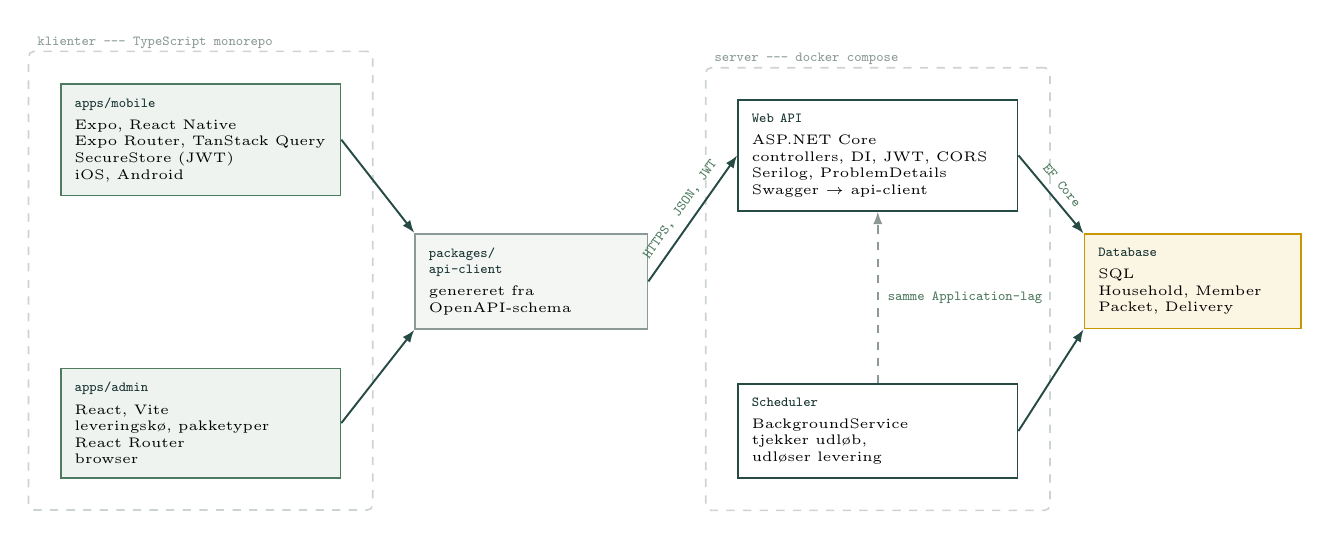
\begin{tikzpicture}
    \node[boxc] (mob) at (0,1.8)
      {\hd{apps/mobile}\\[2pt] Expo, React Native\\ Expo Router, TanStack Query\\ SecureStore (JWT)\\ iOS, Android};
    \node[boxc] (adm) at (0,-1.8)
      {\hd{apps/admin}\\[2pt] React, Vite\\ leveringskø, pakketyper\\ React Router\\ browser};
    \node[boxx,text width=26mm] (cli) at (4.2,0)
      {\hd{packages/}\\ \hd{api-client}\\[2pt] genereret fra\\ OpenAPI-schema};
    \node[box] (api) at (8.6,1.6)
      {\hd{Web API}\\[2pt] ASP.NET Core\\ controllers, DI, JWT, CORS\\ Serilog, ProblemDetails\\ Swagger $\rightarrow$ api-client};
    \node[box] (sch) at (8.6,-1.9)
      {\hd{Scheduler}\\[2pt] BackgroundService\\ tjekker udløb,\\ udløser levering};
    \node[boxd,text width=24mm] (db) at (12.6,0)
      {\hd{Database}\\[2pt] SQL\\ Household, Member\\ Packet, Delivery};

    \begin{scope}[on background layer]
      \node[bnd,fit=(mob)(adm)] (b1) {};
      \node[bnd,fit=(api)(sch)] (b2) {};
    \end{scope}
    \node[bndlbl,above=1mm of b1.north west,anchor=west] {klienter --- TypeScript monorepo};
    \node[bndlbl,above=1mm of b2.north west,anchor=west] {server --- docker compose};

    \draw[ln] (mob.east) -- (cli.north west);
    \draw[ln] (adm.east) -- (cli.south west);
    \draw[ln] (cli.east) -- node[tag,above,sloped] {HTTPS, JSON, JWT} (api.west);
    \draw[ln] (api.east) -- node[tag,above,sloped] {EF Core} (db.north west);
    \draw[ln] (sch.east) -- (db.south west);
    \draw[lnd] (sch.north) -- node[tag,right] {samme Application-lag} (api.south);
  \end{tikzpicture}}
  \bottomnote{Kontrakten mellem klient og server er OpenAPI-schemaet.}
\end{frame}

% ---------- 4 lag (koncept) ----------
\begin{frame}{Hvad er et lag?}{en gruppe klasser med ét fælles ansvar}
  \centering
  \resizebox{0.90\linewidth}{!}{%
  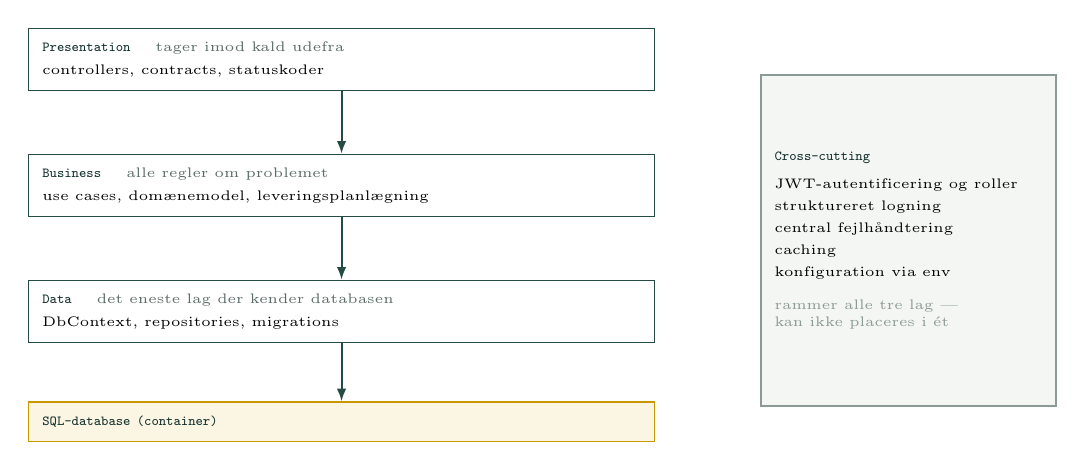
\begin{tikzpicture}
    \node[box,text width=76mm] (l1) at (0,3)
      {\hd{Presentation} \quad {\color{soft}tager imod kald udefra}\\[2pt] controllers, contracts, statuskoder};
    \node[box,text width=76mm] (l2) at (0,1.4)
      {\hd{Business} \quad {\color{soft}alle regler om problemet}\\[2pt] use cases, domænemodel, leveringsplanlægning};
    \node[box,text width=76mm] (l3) at (0,-0.2)
      {\hd{Data} \quad {\color{soft}det eneste lag der kender databasen}\\[2pt] DbContext, repositories, migrations};
    \node[boxd,text width=76mm] (l4) at (0,-1.6)
      {\hd{SQL-database (container)}};
    \draw[ln] (l1) -- (l2);
    \draw[ln] (l2) -- (l3);
    \draw[ln] (l3) -- (l4);
    \node[boxx,text width=34mm,minimum height=42mm] (cc) at (7.2,0.7)
      {\hd{Cross-cutting}\\[4pt]
       JWT-autentificering og roller\\[2pt]
       struktureret logning\\[2pt]
       central fejlhåndtering\\[2pt]
       caching\\[2pt]
       konfiguration via env\\[6pt]
       {\color{faint} rammer alle tre lag ---\\ kan ikke placeres i ét}};
  \end{tikzpicture}}
  \bottomnote{Reglen er hele pointen: \textbf{et lag må kun bruge laget under sig.} Derfor kan vi skifte database uden at røre reglerne, og teste reglerne uden en database.}
\end{frame}

% ---------- 5 lagreglerne ----------
\begin{frame}{Lagreglerne}{står også i CLAUDE.md, så agenten arbejder efter dem}
  \vspace{1mm}
  \scriptsize
  \renewcommand{\arraystretch}{1.35}
  \begin{tabular}{@{}>{\ttfamily\color{deep}}p{22mm}p{52mm}p{45mm}@{}}
    \toprule
    \normalfont\color{soft}\ttfamily modul & \color{soft}\ttfamily må & \color{soft}\ttfamily må ikke \\
    \midrule
    Api & route, validere, mappe contract mod domæne, statuskoder, autorisation & forretningsregler; kende {\ttfamily DbContext} \\
    Application & orkestrere use cases, definere repository-interfaces, transaktionsgrænser & kende HTTP, {\ttfamily ControllerBase}, EF-typer, SQL \\
    Domain & entiteter, invarianter, vandbehov, pakkeindhold, udløb & referere til noget andet projekt overhovedet \\
    Infrastructure & EF-konfiguration, queries, migrations & træffe beslutninger --- den henter og gemmer \\
    clients/apps & kalde API'et via {\ttfamily api-client}, holde UI-state & duplikere forretningsregler; gå uden om klientpakken \\
    \bottomrule
  \end{tabular}
  \bottomnote{Lagene bliver til fire projekter i solution. Næste slide viser hvem der må referere hvem.}
\end{frame}

% ---------- 6 modulafhaengigheder ----------
\begin{frame}{Modulafhængigheder}{de samme fire lag, nu som projekter --- pilen peger mod det, der refereres}
  \centering
  \resizebox{0.88\linewidth}{!}{%
  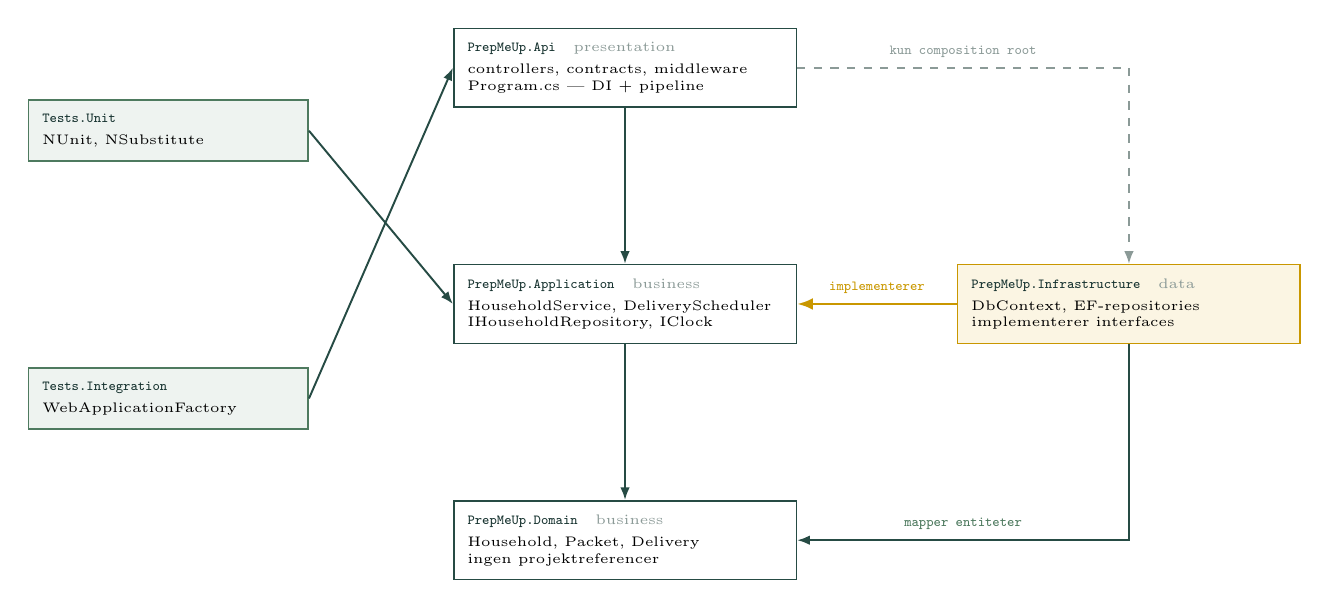
\begin{tikzpicture}
    \node[box,text width=40mm] (apip) at (4,3)
      {\hd{PrepMeUp.Api} \; {\color{faint}presentation}\\[2pt] controllers, contracts, middleware\\ Program.cs --- DI + pipeline};
    \node[box,text width=40mm] (app) at (4,0)
      {\hd{PrepMeUp.Application} \; {\color{faint}business}\\[2pt] HouseholdService, DeliveryScheduler\\ IHouseholdRepository, IClock};
    \node[box,text width=40mm] (dom) at (4,-3)
      {\hd{PrepMeUp.Domain} \; {\color{faint}business}\\[2pt] Household, Packet, Delivery\\ ingen projektreferencer};
    \node[boxd,text width=40mm] (inf) at (10.4,0)
      {\hd{PrepMeUp.Infrastructure} \; {\color{faint}data}\\[2pt] DbContext, EF-repositories\\ implementerer interfaces};
    \node[boxc,text width=32mm] (tu) at (-1.8,2.2)
      {\hd{Tests.Unit}\\[2pt] NUnit, NSubstitute};
    \node[boxc,text width=32mm] (ti) at (-1.8,-1.2)
      {\hd{Tests.Integration}\\[2pt] WebApplicationFactory};

    \draw[ln] (apip) -- (app);
    \draw[ln] (app)  -- (dom);
    \draw[lns] (inf.west) -- node[tag,above,color=signal] {implementerer} (app.east);
    \draw[ln] (inf.south) |- node[tag,above,pos=.75] {mapper entiteter} (dom.east);
    \draw[lnd] (apip.east) -| node[bndlbl,above,pos=.25] {kun composition root} (inf.north);
    \draw[ln] (tu.east) -- (app.west);
    \draw[ln] (ti.east) -- (apip.west);
  \end{tikzpicture}}
  \bottomnote{\textbf{Domain refererer ingenting.} Derfor kan forretningsreglerne testes uden database, browser eller HTTP --- den gule pil vender ind mod domænet i stedet for ud mod databasen.}
\end{frame}

% ---------- 7 EF Core = SQL ----------
\begin{frame}[fragile]{EF Core --- kort fortalt}{I har haft SQL. EF Core skriver SQL'en for jer.}
  \vspace{1mm}
  {\scriptsize\color{soft} En \emph{object-relational mapper}: C\#-klasser bliver til tabeller, og LINQ bliver til SQL. Vi kan altid se den genererede SQL og skrive den i hånden, hvor det er nødvendigt.}
  \vspace{3mm}

  \begin{columns}[T,onlytextwidth]
    \begin{column}{0.47\textwidth}
      {\tiny\ttfamily\color{moss} vi skriver dette i C\#}\\[1mm]
      \begin{semiverbatim}
\tiny\ttfamily
var due = await db.Households
    .Where(h => h.NextDelivery < frist)
    .Include(h => h.Members)
    .ToListAsync();
      \end{semiverbatim}
    \end{column}
    \begin{column}{0.5\textwidth}
      {\tiny\ttfamily\color{moss} EF Core sender dette til databasen}\\[1mm]
      \begin{semiverbatim}
\tiny\ttfamily
SELECT h.*, m.*
FROM Households AS h
LEFT JOIN HouseholdMembers AS m
     ON m.HouseholdId = h.Id
WHERE h.NextDelivery < @frist
      \end{semiverbatim}
    \end{column}
  \end{columns}

  \vspace{2mm}
  \tiny
  \renewcommand{\arraystretch}{1.2}
  \begin{tabular}{@{}>{\ttfamily\color{deep}}p{38mm}p{42mm}p{45mm}@{}}
    \toprule
    \normalfont\color{soft}\ttfamily i C\# & \color{soft}\ttfamily i SQL & \color{soft}\ttfamily bemærk \\
    \midrule
    class Household        & {\ttfamily CREATE TABLE Households} & én klasse, én tabel \\
    List$<$Member$>$ Members & fremmednøgle + {\ttfamily JOIN}    & kaldes en navigation \\
    SaveChangesAsync()     & {\ttfamily INSERT}/{\ttfamily UPDATE} i én transaktion & alt eller intet \\
    migration              & versionsstyrede {\ttfamily ALTER TABLE}-scripts & ligger i git \\
    \bottomrule
  \end{tabular}
\end{frame}

% ---------- 8 sekvens ----------
\begin{frame}{Ét kald gennem stakken}{POST /api/households}
  \centering
  \resizebox{0.95\linewidth}{!}{%
  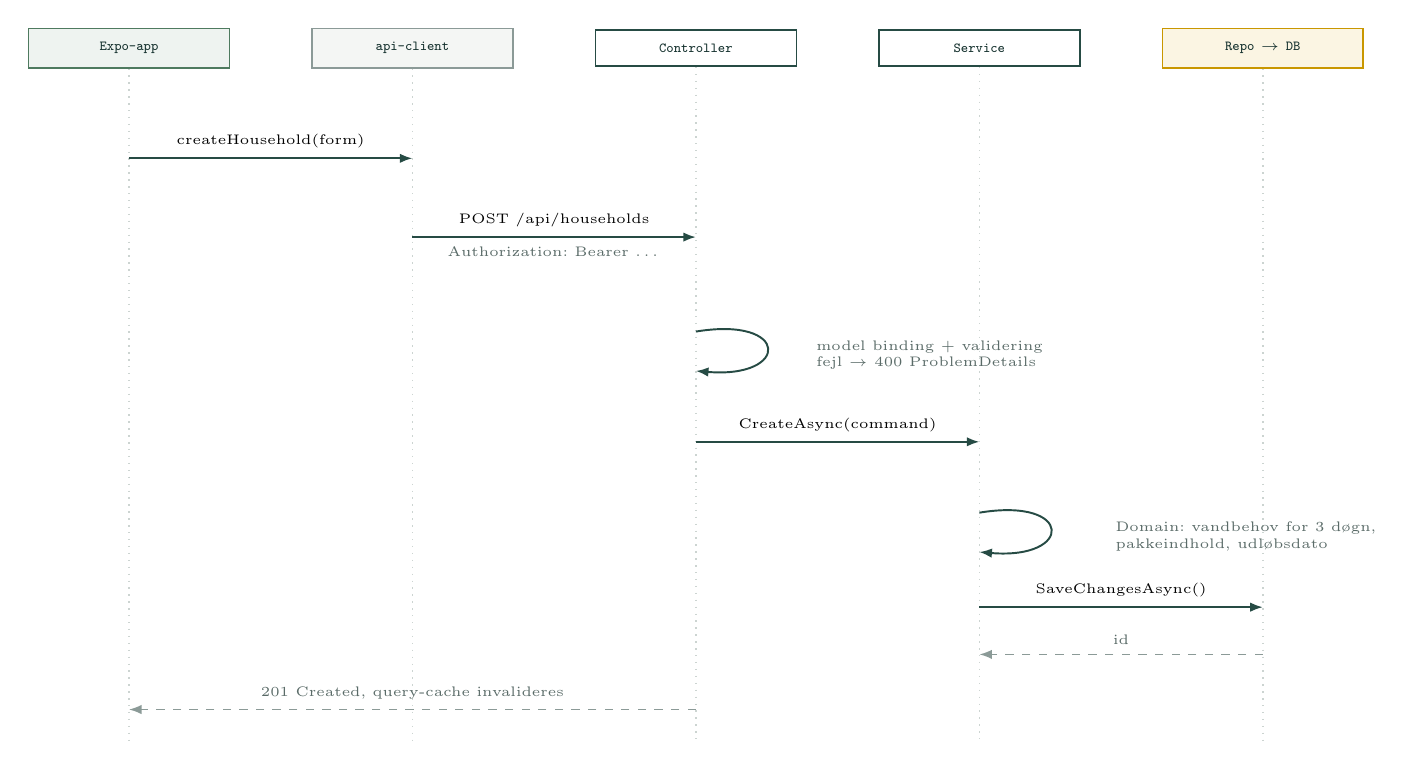
\begin{tikzpicture}[font=\tiny]
    \def\yT{0} \def\yB{-8.6}
    \node[boxc,text width=22mm,align=center] (c1) at (0,\yT)  {\hd{Expo-app}};
    \node[boxx,text width=22mm,align=center] (c2) at (3.6,\yT) {\hd{api-client}};
    \node[box, text width=22mm,align=center] (c3) at (7.2,\yT) {\hd{Controller}};
    \node[box, text width=22mm,align=center] (c4) at (10.8,\yT){\hd{Service}};
    \node[boxd,text width=22mm,align=center] (c5) at (14.4,\yT){\hd{Repo $\rightarrow$ DB}};

    \foreach \n in {c1,c2,c3,c4,c5} \draw[life] (\n.south) -- ($(\n.south)+(0,\yB)$);

    \draw[ln] (0,-1.4) -- node[above]{createHousehold(form)} (3.6,-1.4);
    \draw[ln] (3.6,-2.4) -- node[above]{POST /api/households} node[below,color=soft]{Authorization: Bearer \ldots} (7.2,-2.4);
    \draw[ln] (7.2,-3.6) .. controls (8.4,-3.4) and (8.4,-4.2) .. (7.2,-4.1)
          node[right,xshift=14mm,yshift=2mm,color=soft,align=left]{model binding + validering\\ fejl $\rightarrow$ 400 ProblemDetails};
    \draw[ln] (7.2,-5.0) -- node[above]{CreateAsync(command)} (10.8,-5.0);
    \draw[ln] (10.8,-5.9) .. controls (12.0,-5.7) and (12.0,-6.5) .. (10.8,-6.4)
          node[right,xshift=16mm,yshift=2mm,color=soft,align=left]{Domain: vandbehov for 3 døgn,\\ pakkeindhold, udløbsdato};
    \draw[ln] (10.8,-7.1) -- node[above]{SaveChangesAsync()} (14.4,-7.1);
    \draw[lnd] (14.4,-7.7) -- node[above,color=soft]{id} (10.8,-7.7);
    \draw[lnd] (7.2,-8.4) -- node[above,color=soft]{201 Created, query-cache invalideres} (0,-8.4);
  \end{tikzpicture}}
  \bottomnote{Læg mærke til, at kaldet går præcis én vej ned gennem lagene og samme vej tilbage.}
\end{frame}

% ---------- 9 deployment ----------
\begin{frame}{Deployment}{udviklingsopsætning}
  \centering
  \resizebox{0.82\linewidth}{!}{%
  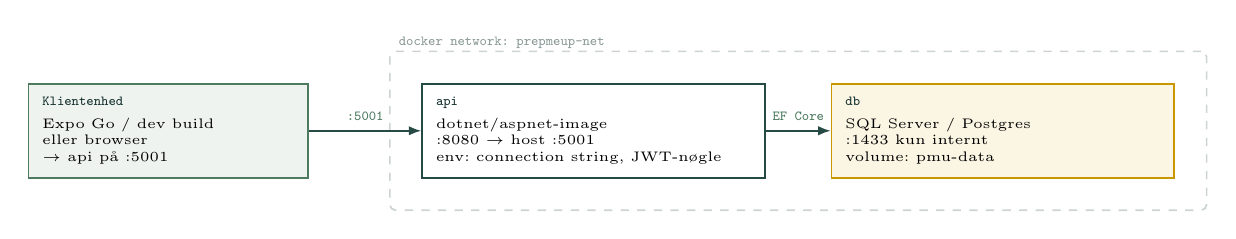
\begin{tikzpicture}
    \node[boxc,text width=32mm] (cl) at (0,0)
      {\hd{Klientenhed}\\[2pt] Expo Go / dev build\\ eller browser\\ $\rightarrow$ api på :5001};
    \node[box,text width=40mm] (api) at (5.4,0)
      {\hd{api}\\[2pt] dotnet/aspnet-image\\ :8080 $\rightarrow$ host :5001\\ env: connection string, JWT-nøgle};
    \node[boxd,text width=40mm] (db) at (10.6,0)
      {\hd{db}\\[2pt] SQL Server / Postgres\\ :1433 kun internt\\ volume: pmu-data};
    \begin{scope}[on background layer]
      \node[bnd,fit=(api)(db)] (net) {};
    \end{scope}
    \node[bndlbl,above=1mm of net.north west,anchor=west] {docker network: prepmeup-net};
    \draw[ln] (cl) -- node[tag,above]{:5001} (api);
    \draw[ln] (api) -- node[tag,above]{EF Core} (db);
  \end{tikzpicture}}
  \bottomnote{Databasen eksponeres ikke til host --- kun \texttt{api} når den, via servicenavnet \texttt{db}. Derfor er opsætningen ens på Windows og Linux. Logning skrives med Serilog til fil og database (BAD, lektion 7).}
\end{frame}

% ---------- 10 repoet ----------
\begin{frame}[fragile]{Repoet}{mapperne under src/ svarer 1:1 til modulerne}
  \vspace{1mm}
\begin{semiverbatim}
\tiny\ttfamily
prepmeup/
|-- CLAUDE.md                     \color{faint}# lagregler, konventioner, definition of done\color{deep}
|-- .claude/
|   |-- settings.json             \color{faint}# naegter adgang til .env og noeglefiler\color{deep}
|   |-- agents/                   \color{faint}# 10 specialiserede reviewere\color{deep}
|   `-- skills/                   \color{faint}# 8 arbejdsgange\color{deep}
|-- src/
|   |-- PrepMeUp.Domain/          \color{moss}// ingen referencer\color{deep}
|   |-- PrepMeUp.Application/     \color{moss}// interfaces + use cases\color{deep}
|   |-- PrepMeUp.Infrastructure/  \color{moss}// EF Core\color{deep}
|   `-- PrepMeUp.Api/             \color{moss}// HTTP + BackgroundService\color{deep}
|-- clients/
|   |-- CLAUDE.md                 \color{faint}# TS strict, ingen forretningslogik i UI\color{deep}
|   |-- apps/mobile/              \color{faint}# Expo\color{deep}
|   |-- apps/admin/               \color{faint}# React + Vite\color{deep}
|   `-- packages/api-client/      \color{faint}# genereret - redigeres ikke i haanden\color{deep}
|-- tests/
|   |-- PrepMeUp.Tests.Unit/
|   `-- PrepMeUp.Tests.Integration/
|-- docs/adr/                     \color{faint}# beslutningsreferater til eksamen\color{deep}
|-- docker-compose.yml
`-- .gitlab-ci.yml
\end{semiverbatim}
\end{frame}

% ---------- 11 udviklingsopsaetning ----------
\begin{frame}{Udviklingsopsætning}{værktøj omkring repoet --- kører ikke i produktion}
  \centering
  \resizebox{0.95\linewidth}{!}{%
  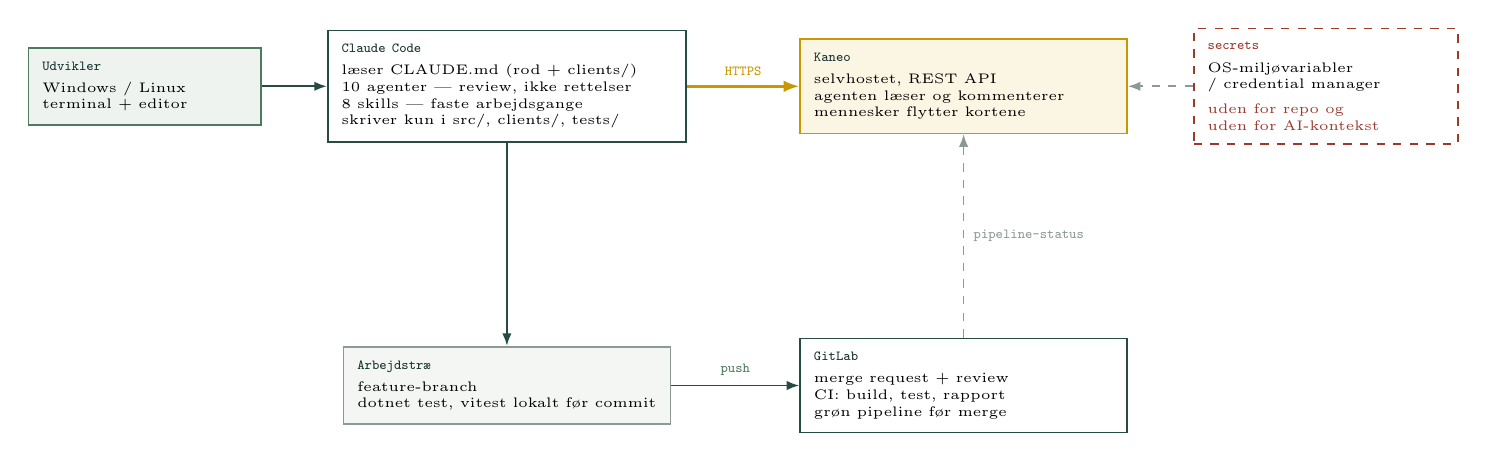
\begin{tikzpicture}
    \node[boxc,text width=26mm] (dev) at (0,1.4)
      {\hd{Udvikler}\\[2pt] Windows / Linux\\ terminal + editor};
    \node[box,text width=42mm] (cc) at (4.6,1.4)
      {\hd{Claude Code}\\[2pt] læser CLAUDE.md (rod + clients/)\\ 10 agenter --- review, ikke rettelser\\ 8 skills --- faste arbejdsgange\\ skriver kun i src/, clients/, tests/};
    \node[boxx,text width=38mm] (wt) at (4.6,-2.4)
      {\hd{Arbejdstræ}\\[2pt] feature-branch\\ dotnet test, vitest lokalt før commit};
    \node[box,text width=38mm] (gl) at (10.4,-2.4)
      {\hd{GitLab}\\[2pt] merge request + review\\ CI: build, test, rapport\\ grøn pipeline før merge};
    \node[boxd,text width=38mm] (kn) at (10.4,1.4)
      {\hd{Kaneo}\\[2pt] selvhostet, REST API\\ agenten læser og kommenterer\\ mennesker flytter kortene};
    \node[draw=alert,dashed,line width=.6pt,text width=30mm,align=left,inner sep=5pt,font=\tiny] (sec) at (15.0,1.4)
      {{\ttfamily\bfseries\color{alert}secrets}\\[2pt] OS-miljøvariabler\\ / credential manager\\[3pt] {\color{alert}uden for repo og\\ uden for AI-kontekst}};

    \draw[ln] (dev) -- (cc);
    \draw[ln] (cc.south) -- (wt.north);
    \draw[ln] (wt) -- node[tag,above]{push} (gl);
    \draw[lns] (cc.east) -- node[tag,above,color=signal]{HTTPS} (kn.west);
    \draw[lnd] (sec.west) -- (kn.east);
    \draw[lnd] (gl.north) -- node[bndlbl,right]{pipeline-status} (kn.south);
  \end{tikzpicture}}
  \bottomnote{Tokenet kommer fra miljøet --- aldrig fra en fil, agenten kan læse.}
\end{frame}

% ---------- 12 agenterne ----------
\begin{frame}{Agenterne}{ti specialister --- alle read-only på nær adr-scribe}
  \vspace{1mm}
  \tiny
  \renewcommand{\arraystretch}{1.4}
  \begin{tabular}{@{}>{\ttfamily\color{deep}}p{30mm}p{60mm}p{34mm}@{}}
    \toprule
    \normalfont\color{soft}\ttfamily agent & \color{soft}\ttfamily rolle & \color{soft}\ttfamily kaldes \\
    \midrule
    architecture-guardian & fanger brud på lagreglerne og afhængighedsretningen & før hver merge request \\
    api-designer          & ressourcenavne, verber, statuskoder, contracts & før et endpoint bygges \\
    test-designer         & testtilfælde med ækvivalensklasser og grænseværdier & før tests skrives \\
    data-modeler          & EF-model, relationer, normalisering, N+1 & ved ændring i datamodellen \\
    frontend-reviewer     & hooks, typer, loading/tom/fejl, logik i klienten & ved klientændringer \\
    refactoring-scout     & design smells til konkret refactoring med pris & ved iterationsafslutning \\
    security-reviewer     & auth, adgangskontrol, hemmeligheder, validering & før deployment \\
    adr-scribe            & beslutningsreferater i docs/adr & når en beslutning er truffet \\
    integration-planner   & afhængighedstræ og integrationsplan & før integrationstest \\
    oral-examiner         & eksaminerer jer i jeres eget projekt & før eksamen \\
    \bottomrule
  \end{tabular}
\end{frame}

% ---------- 13 skills ----------
\begin{frame}{Skills}{otte faste arbejdsgange}
  \vspace{2mm}
  \scriptsize
  \renewcommand{\arraystretch}{1.3}
  \begin{tabular}{@{}>{\ttfamily\color{deep}}p{32mm}p{95mm}@{}}
    \toprule
    \normalfont\color{soft}\ttfamily skill & \color{soft}\ttfamily hvad den gør \\
    \midrule
    vertical-slice   & ny funktion gennem alle fire lag i rigtig rækkefølge --- Domain først \\
    tdd-loop         & red-green-refactor med NUnit og NSubstitute \\
    api-contract     & holder OpenAPI-schema og api-client i sync \\
    expo-screen      & ny skærm med routing, query og alle fire tilstande \\
    git-flow         & branch, commit, pull--test--push, merge request \\
    kaneo            & læser og kommenterer opgaver via API'et \\
    domain-modelling & faciliterer domænemodellen med spørgsmål \\
    report-check     & tegngrænse, kapitelstruktur, skriveregler \\
    \bottomrule
  \end{tabular}
\end{frame}

% ---------- 14 graenser ----------
\begin{frame}{Grænserne vi har sat}{tre bevidste begrænsninger på hvad agenten må}
  \vspace{3mm}
  \begin{itemize}\setlength\itemsep{5mm}
    \punkt{Agenterne retter ikke koden}{De rapporterer fund med fil, linje og forslag. Et fund du selv retter, er et fund du kan forklare til eksamen.}
    \punkt{Testdesign er delt i to}{\texttt{test-designer} foreslår testtilfældene og begrunder dem. Først når et menneske har godkendt listen, implementerer \texttt{tdd-loop} dem. Testdesign er et læringsmål i softwaretest.}
    \punkt{Kaneo-agenten flytter ikke kort}{Den læser og kommenterer. Statusskift er gruppens beslutning --- den iterative proces er et læringsmål, og tavlens historik bliver procesbilag i rapporten.}
  \end{itemize}
  \bottomnote{Samme princip i \texttt{domain-modelling} og \texttt{report-check}: de stiller spørgsmål og kritiserer, men producerer hverken modellen eller rapportprosaen.}
\end{frame}

% ---------- 15 ordforklaring ----------
\begin{frame}{Tre ord der er faldet undervejs}{}
  \vspace{3mm}
  \begin{itemize}\setlength\itemsep{5mm}
    \punkt{Vertical slice}{Vi bygger én funktion hele vejen igennem --- fra skærm til database --- frem for ét lag ad gangen. Hver iteration ender med noget, der virker, i stedet for tre færdige lag og ingen funktion.}
    \punkt{Clean Architecture}{Et udbredt navn for den lagdeling, vi bruger, hvor afhængighederne peger ind mod domænet. Kurset kalder det \emph{Layers} --- og det er kursets ord, vi bruger i rapporten.}
    \punkt{MediatR}{Et bibliotek, der lægger et mellemled ind mellem controller og logik. \textbf{Vi bruger det ikke:} det løser et problem, vi ikke har endnu, og det står ikke i pensum.}
  \end{itemize}
\end{frame}

\end{document}